\documentclass[a4paper, 12pt]{article}
\usepackage{pgfplots}

\begin{document}

\section{From File}
\begin{figure}[h]
  \centering
  \begin{tikzpicture}
    \begin{axis}[
      width=\textwidth,
      axis x line=middle,
      axis y line=middle,
      enlargelimits=0.2,
      ultra thick,
      blue!50!black
      ]

      \addplot+[
      ultra thick,
      purple,
      mark=*,
      mark options={scale=1.25}
      ]
      table{data/sinx.dat};

    \end{axis}
  \end{tikzpicture}
  \caption{$\sin(x)$ from file}
\end{figure}
\pagebreak

\section{Direct}
\begin{figure}[h]
  \centering
  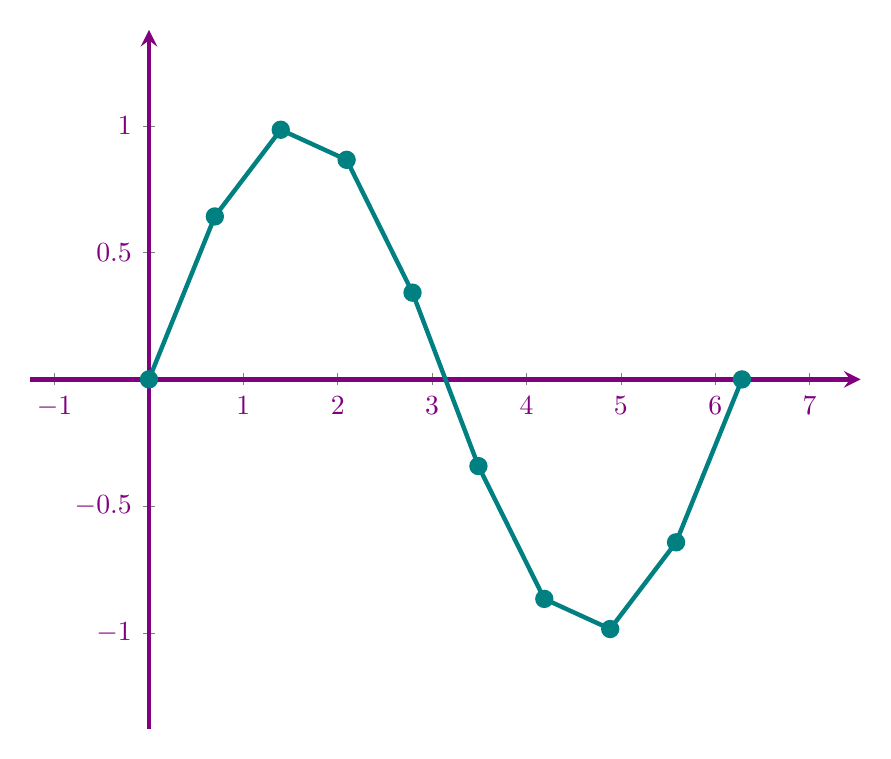
\begin{tikzpicture}
    \begin{axis}[
      width=\textwidth,
      axis x line=middle,
      axis y line=middle,
      enlargelimits=0.2,
      ultra thick,
      violet,
      ]

      \addplot+[
      ultra thick,
      green!50!blue,
      mark=*,
      mark options={scale=1.25},
      samples=10,
      domain=0:2*pi
      ]
      {sin(deg(x))};

    \end{axis}
  \end{tikzpicture}
  \caption{$\sin(x)$ directly}
\end{figure}
\pagebreak

\section{Noise Added}
\begin{figure}[h]
  \centering
  \begin{tikzpicture}
    \begin{axis}[
      width=\textwidth,
      axis x line=middle,
      axis y line=middle,
      enlargelimits=0.2,
      ultra thick,
      green!20!blue!50!black,
      % violet,
      ]

      \addplot+[
      ultra thick,
      orange!90,
      mark=none,
      domain=0:2*pi,
      ]
      {sin(deg(x))};

      \addplot+[
      only marks,
      mark=*,
      mark options={violet!80!black},
      ]
      table{data/noise-sinx.dat};
    \end{axis}
  \end{tikzpicture}
  \caption{$\sin(x)$ from file with noise added}
\end{figure}

\end{document}
